\documentclass{article}
\usepackage{authblk}
\usepackage{acro}
\usepackage{amsmath}
\usepackage{amsfonts}
\usepackage{caption}
\usepackage{ccaption}
\usepackage[margin=20truemm]{geometry}
\usepackage[dvipdfmx]{graphicx}
\usepackage{hyperref}
\usepackage{url}

\title{
  A graph-based practice of evaluating collective idendities of cell clusters
}
\author[1,2]{Yuji Okano}
\author[2]{Yoshitaka Kase}
\author[2]{Hideyuki Okano}
\affil[1]{
  Department of Extended Intelligence for Medicine, 
  The Ishii-Ishibashi Laboratory, 
  Keio University School of Medicine
}
\affil[2]{
  Division of CNS Regeneration and Drug Discovery,
  International Center for Brain Science, 
  Fujita Health University
}
\date{\today}

\DeclareAcronym{scRNA-seq}{short = scRNA-seq, long  = single-cell RNA-sequencing}
\DeclareAcronym{GRN}{short = GRN, long  = gene regulatory network}
\DeclareAcronym{JIM}{short = JIM, long  = Jaccard index matrix}
\DeclareAcronym{DEA}{short = DEA, long  = differential expression analysis}
\DeclareAcronym{DEG}{short = DEG, long  = differentially expressed gene}

\DeclareCaptionLabelFormat{mainfigs}{\textbf{Figure #2}}
\captionsetup[figure]{labelformat=mainfigs}

\urlstyle{same}

\begin{document}

\maketitle

\section*{Abstract}
Random sentences

\section*{Introduction}
It has been more than 10 years since the birth of \ac{scRNA-seq}, and the technology 
now is recognized as a prominent game changer of modern molecular biology. Likewise the pioneering technology, 
bulk RNA-seq,
scRNA-seq can observe multidimensional gene expression profiles, while
it also can provide such information in single-cell-level.

$\vdots$

In our previous research, we proposed a \ac{GRN}-based
representation of cell clusters while edges of GRNs explain statistical
dependencies between two genes, and demonstrated that similarity of
two clusters can be defined as a quasi-pseudo-metric function $d^*$\cite{okano2023set}. When the 

In addition to the theoretical proposal, we applied our logic to 
the annotation of scRNA-seq data, and showed that the GRN-based anntation can visualize the similarities and the
difference of cell clusters, which the conventional \ac{DEG}-based manual annotation could not address due to the objectives of \ac{DEA} to summerize the biological semantics 
of the clusters. Althogh we introduced a theory to form GRNs based on dependencies of gene expressions, we 
compromised to implement the algorithm relying on the statistical test of 
correlation to deal with the continuity of scRNA-seq data. Considering the fact that 
our method's primary application is the annotation of scRNA-seq data, 
an effective binarization method is needed to reduce computational costs and 
streamline the overall time required to initiate main analyses. Furthermore, we 
intended to make our framework dependent on researchers' expertises on the 
sample domains so that the metrics of cellular identities are tailor-made for the 
research scopes providing necessary and sufficient resolutions. Constrary, this 
design made our algorithm unfriendly to users. As the legitimacy our theory 
needs to be validated in various cases, A semi-automated system to help users 
select key marker genes is desired.

\begin{figure}[htb]
  \centering
  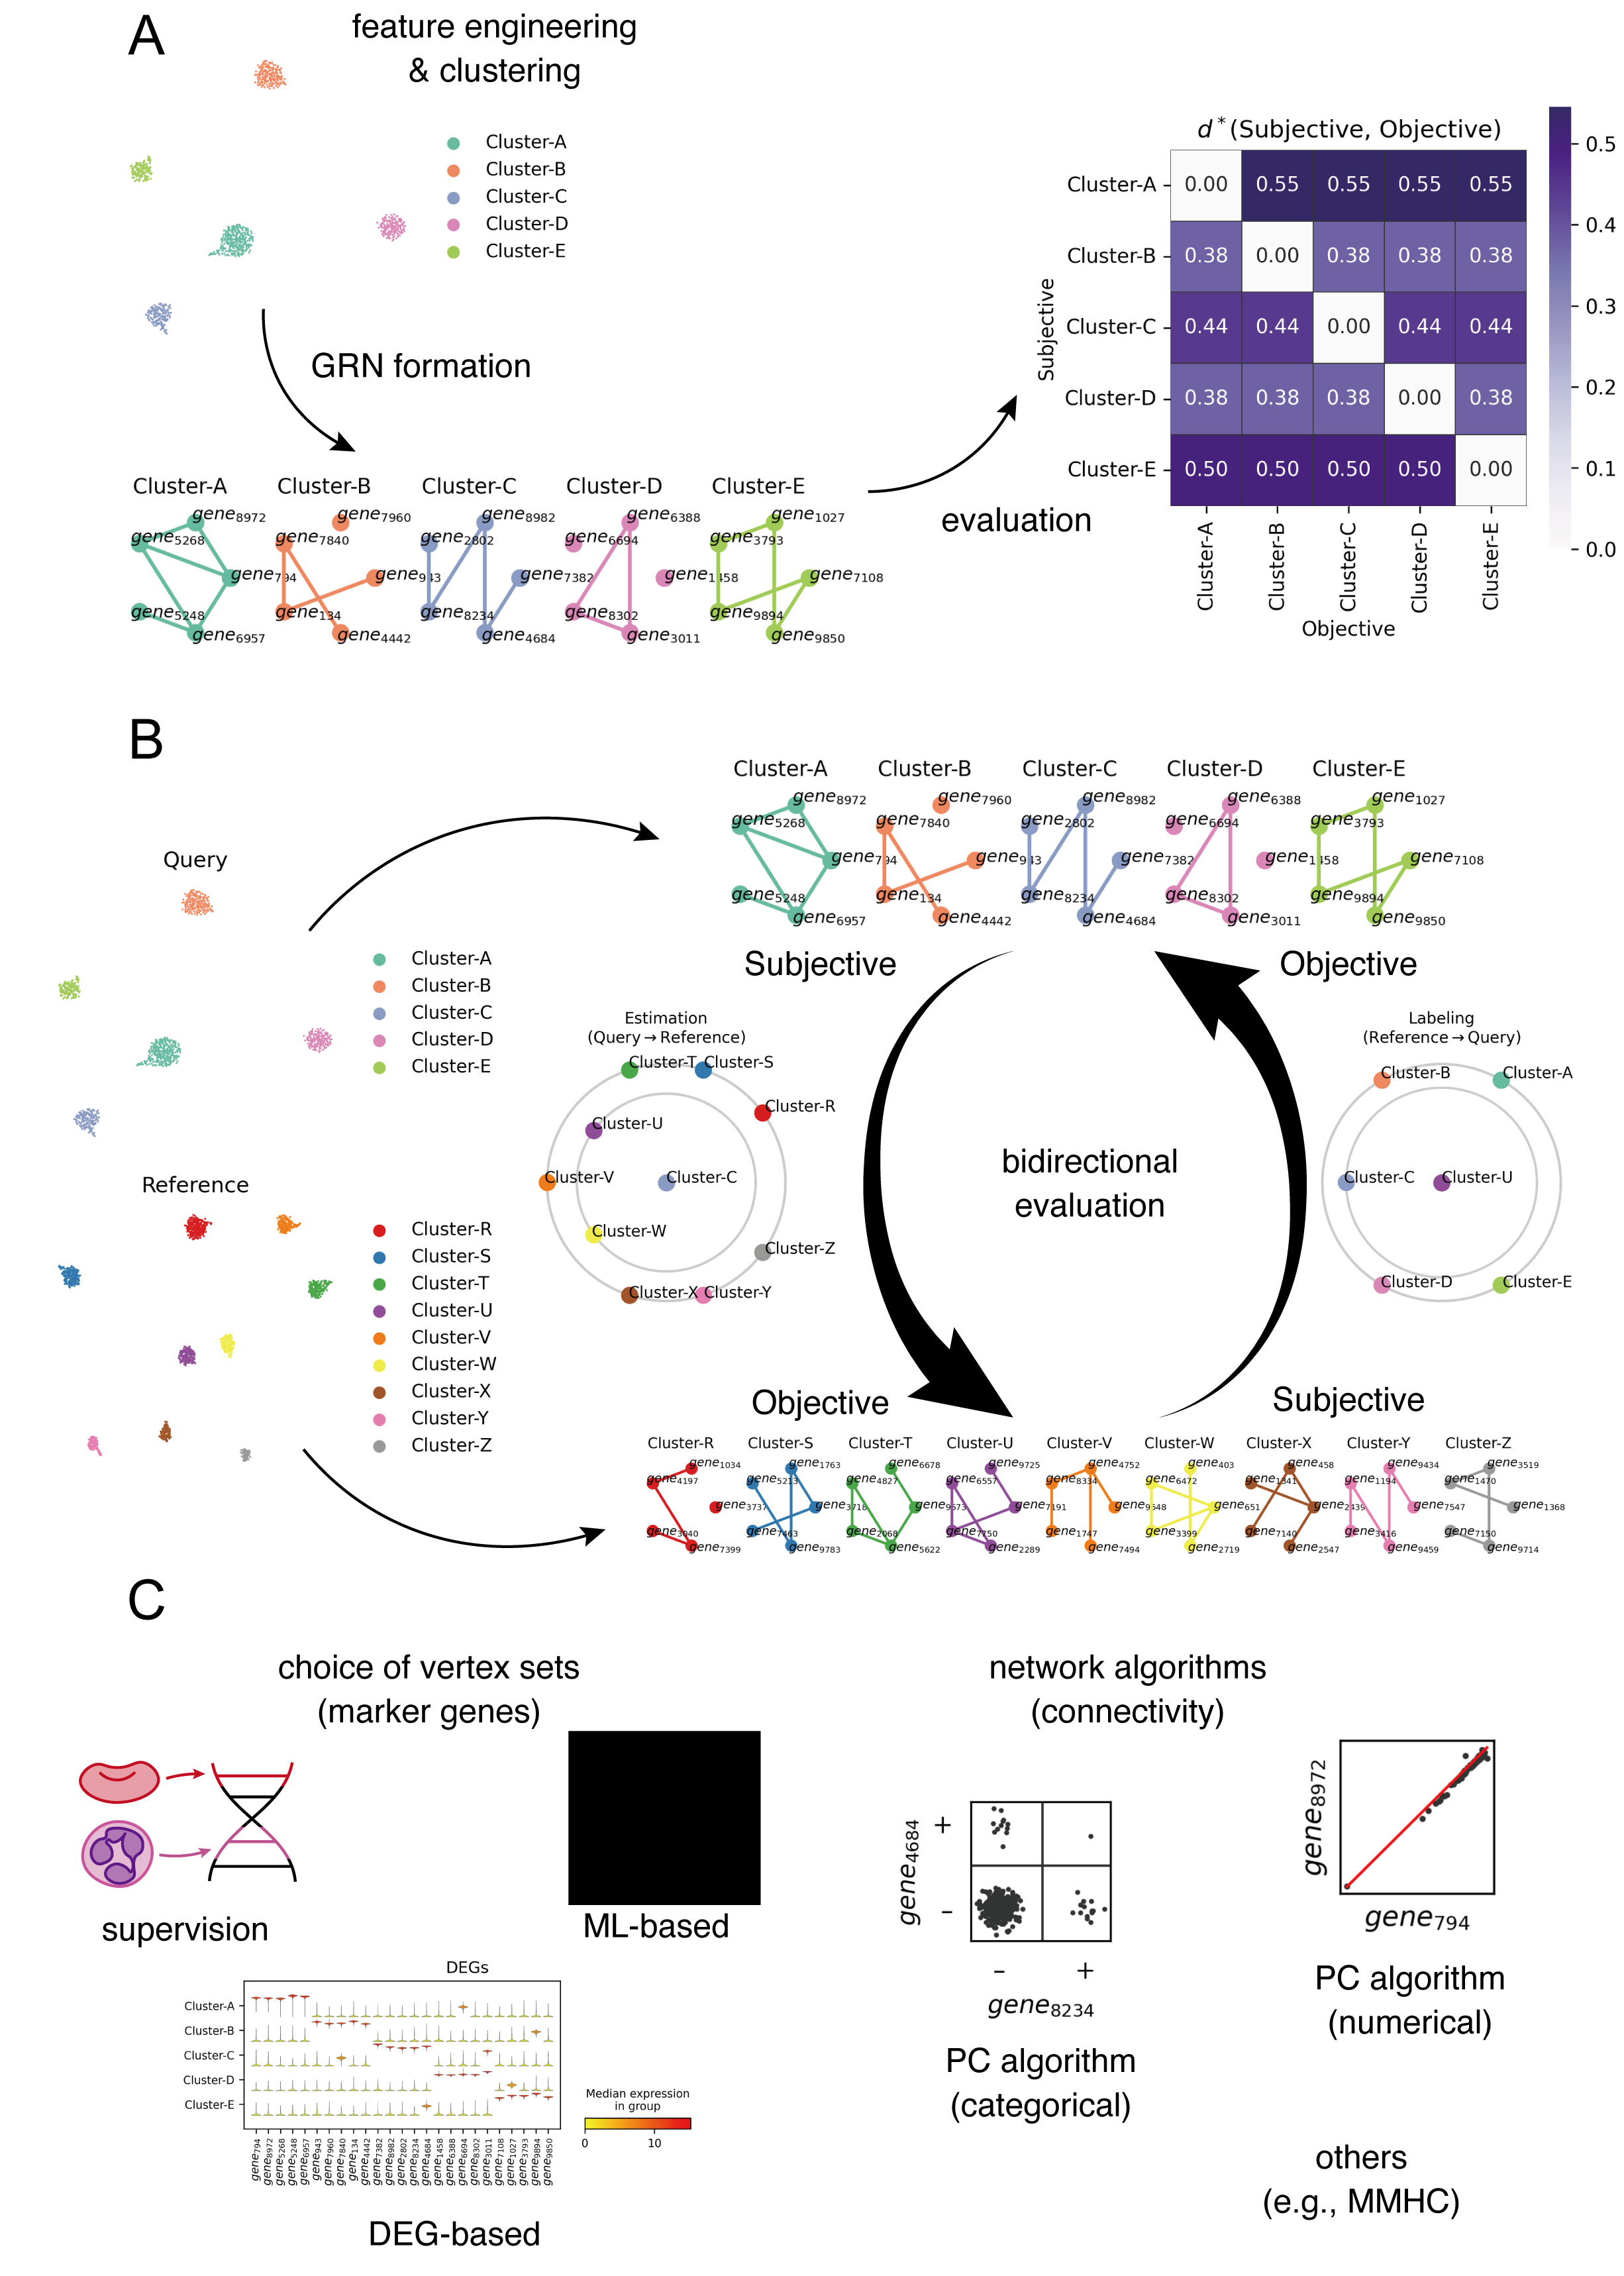
\includegraphics[scale=0.7]{./figs/exported/figure_1.png}
  \caption{The framework of the GRN-based characterization and annotation of cell classes}
  \legend{
    \textbf{A}: The foundation of the GRN-based characterization of cell classes. 
    After clustering in designed data space by arbitrary methods, cell classes (the clusters) can be represented by 
    GRNs of corresponding genes of choice. The similarity of two GRNs of the same vertex 
    (marker gene) are evaluated with the assymetrical function $d^*$, where the return values 
    reflects the similarity from the viewpoint of the subjective clusters. \textbf{B}: 
    Schematic of the GRN-based scRNA-seq data annotation. Expecting the referential data to reflect canonical 
    states of target sample domains, the evaluation of the similarity among cell classes can be performed bidirectionally.
    \textbf{C}: Methodological variations of the selection of vertex sets (marker genes) and the algorithms to compute the network structures of GRNs.
  }
  \label{framework}
\end{figure}

$\vdots$

Leveraging the backbone theory of GRN-based comparisons of cluster-wise
cellular identities (i.e., cell classes), we implemented 

$\vdots$

To simplify the contents of this study to highlight our foci, we would not 
discuss any practices of designing data spaces or clustering in depth.

\section*{Results}
\subsection*{Challenges of the framework of GRN-based methods}
In this reserch, we revisited the workflow of the GRN-based annotation


\subsection*{Automated marker-gene suggestion}
Although we intended to require experimenters to curate marker genes to use
in GRNs, overly recurrsive trials to find 

\begin{figure}[htb]
  \centering
  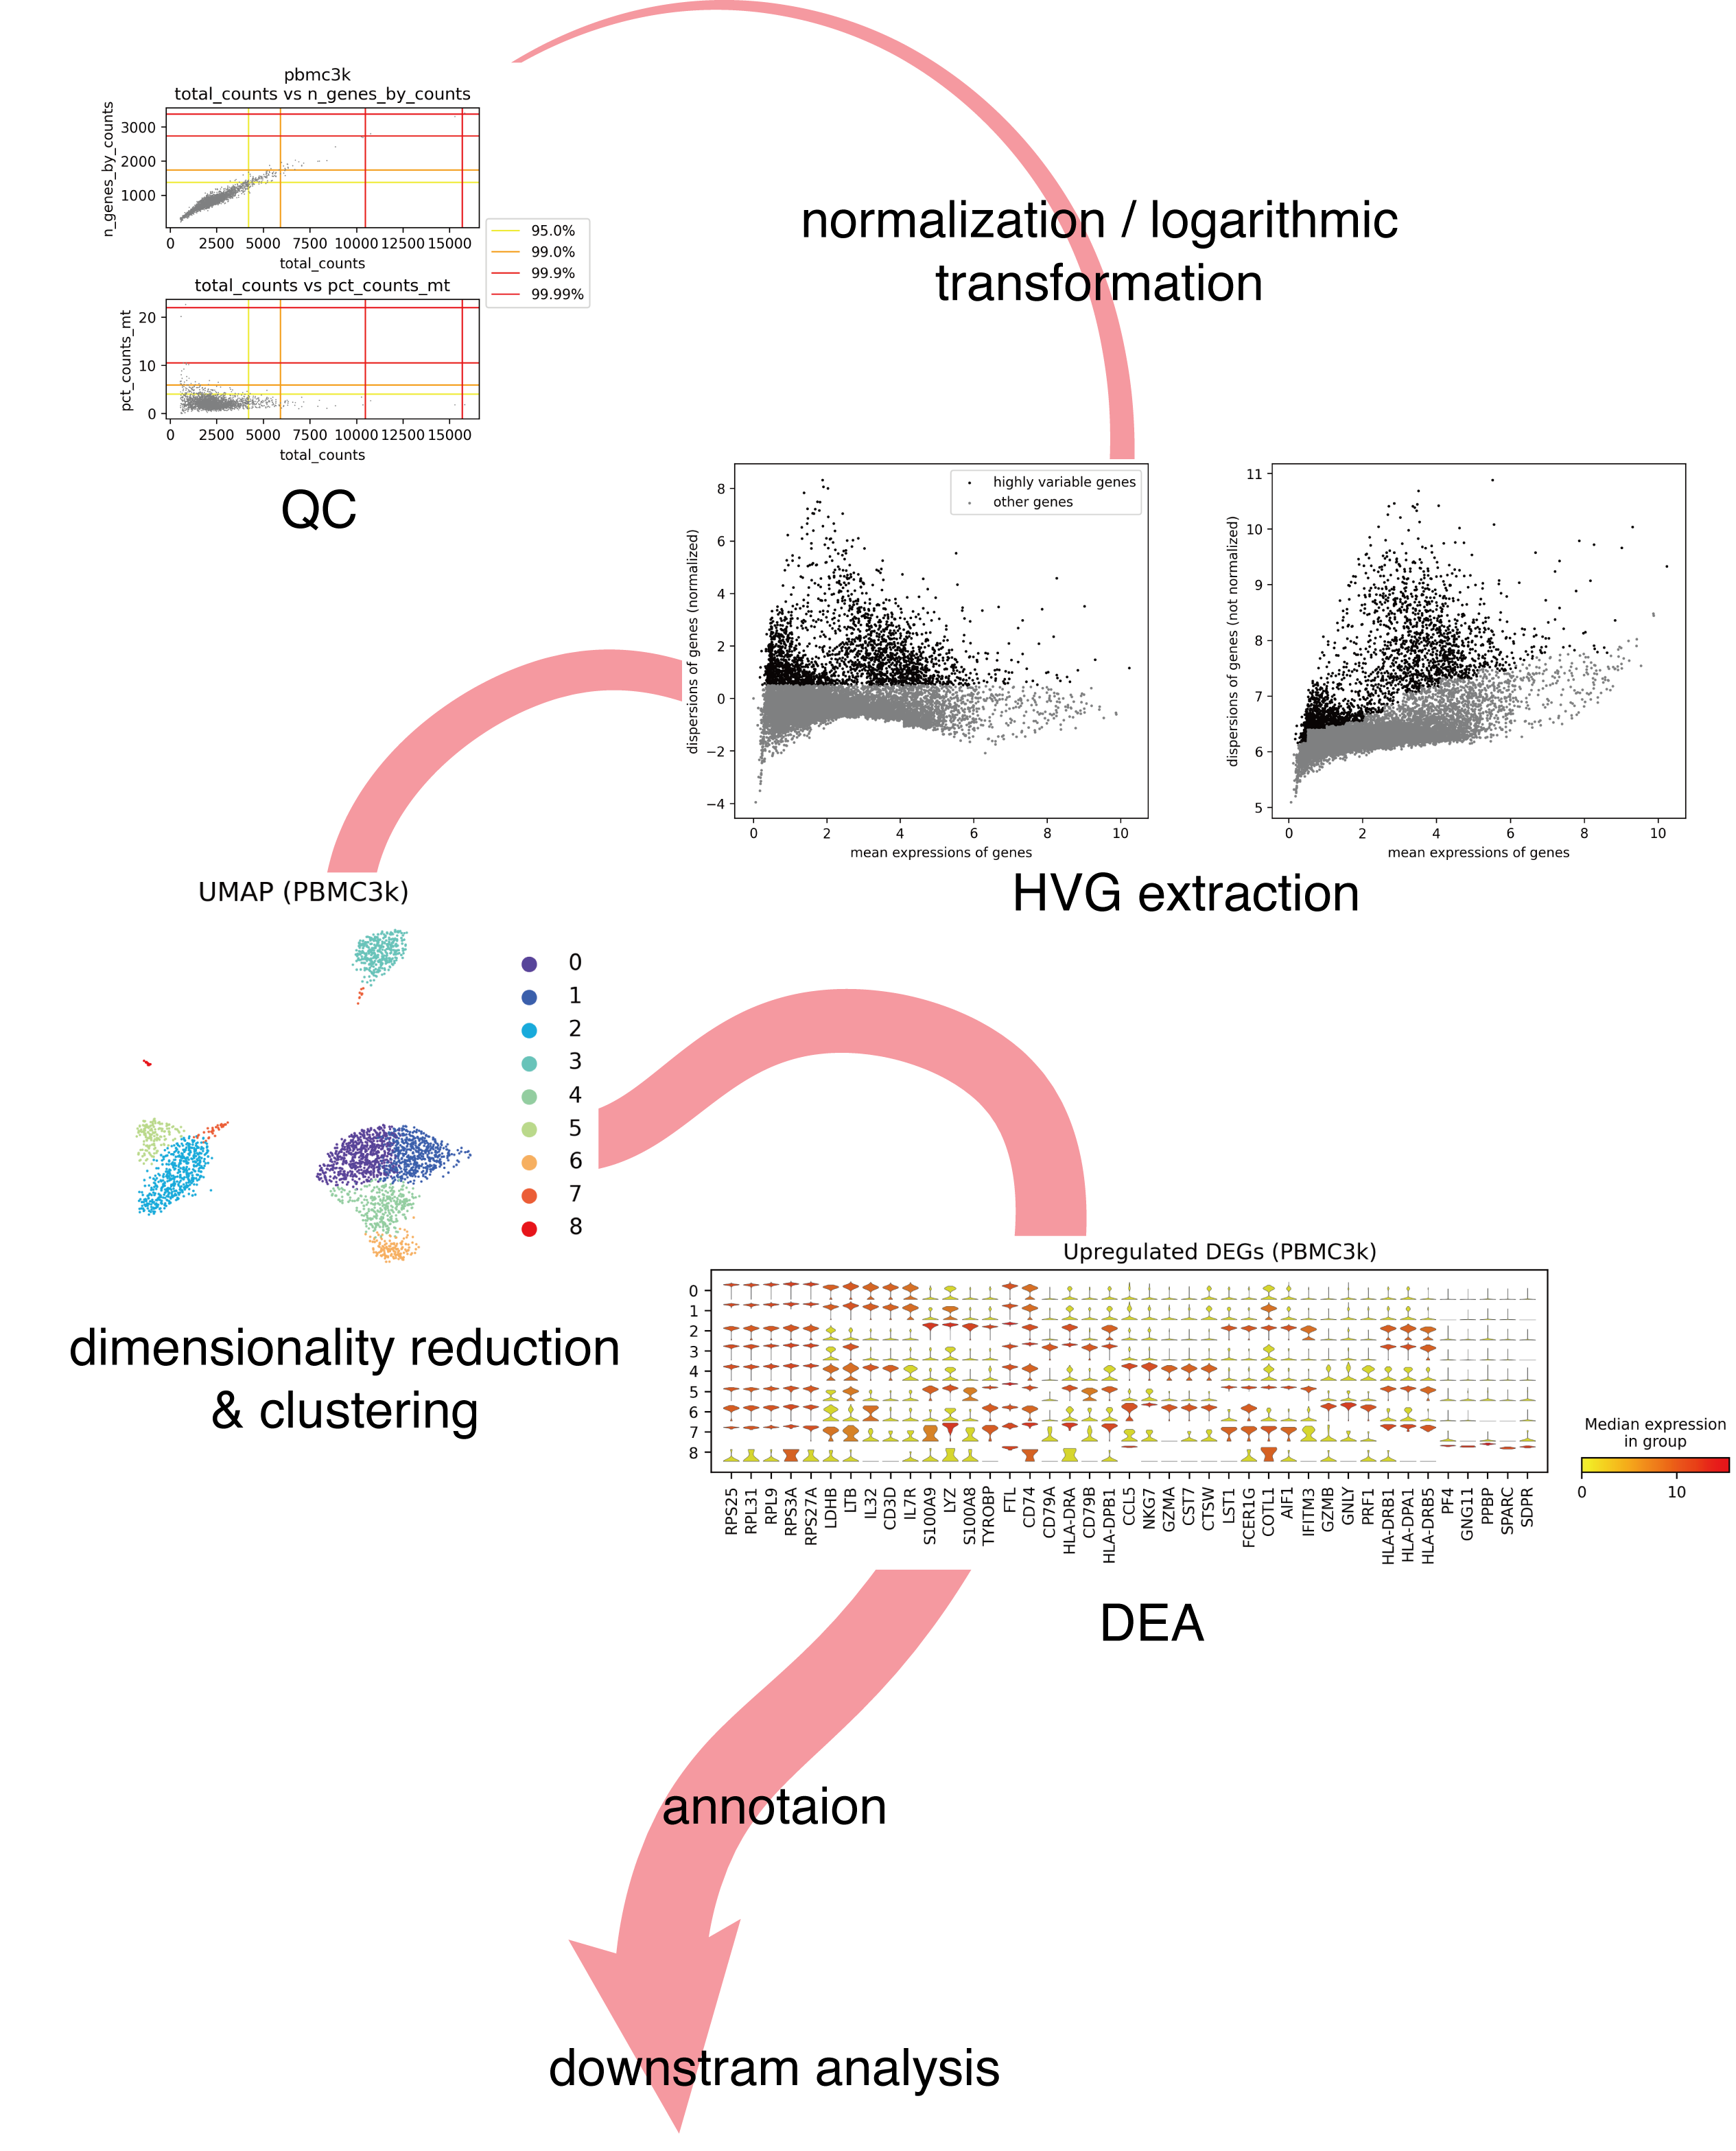
\includegraphics[scale=0.6]{./figs/exported/figure_s1.png}
  \caption{Gene expression patterns of clusters in PBMC3k}
  \label{bc}
\end{figure}


\subsection*{Dropout-based binarization}
\subsection*{Benchmarking}

\section*{Discussion}
I have no idea.

\section*{Methods}
\subsection*{GRNet Impletemtations}

\subsubsection*{GO term-assisted gene selection referring Jaccard Index}
\begin{equation}\label{jaccard}
  J(A, B) := \frac{A\cap B}{A\cup B}
\end{equation}
Jaccard Index of two sets $A, B$ is defined as Eq. \eqref{jaccard}. We expanded this 
definition to pairwise comparisons of multiple elements by forming a matrix 
where each element is the corresponding Jaccard Index, and we named the matrix \ac{JIM}. For example, the element in 
$i$-th row and $j$-th column (where $i, j, k\in\mathbb{N}$ and $i\leq k, j\leq k$), $JIM_{i,j}$, can be defined as
follows when a JIM of sets $X_1, X_2,\cdots, X_k$ are considered:
\begin{equation}\label{jim}
  JIM_{i, j} := J(X_i, X_j)
\end{equation}
Especially for seed markers, sets of subscribed GO terms (let $G_1, \cdots, G_k$)
and their JIM are calulated in order to set $min_{i,j}(J(G_i, G_j))$ as a threshold of 
biological correspondence.

$\vdots$

For detailed method of implementation, we calculated the JIM of the related GO terms of given seed markers. We used mygene.py\cite{mygene} to query the GO database, and Numpy\cite{numpy} to calculate JIM.

\subsubsection*{GRNs and the evaluation function}
Following our previous report\cite{okano2023set}, we computed GRNs by calculating
correlations of continuous gene expression values (e.g., $log_2(RPM+1)$) using Pgmpy\cite{pgmpy}. In this study, we introduced

\subsection*{scRNA-seq data analysis}
\subsubsection*{Dataset List}
The scRNA-seq data we used in this research were publicly available as online
resources as follows:\\
M1C10X: \url{https://portal.brain-map.org/atlases-and-data/rnaseq/human-m1-10x}\\
hFB: \url{https://www.ncbi.nlm.nih.gov/geo/query/acc.cgi?acc=GSE165388}\\
PBMC3k: \url{https://support.10xgenomics.com/single-cell-gene-expression/datasets/1.1.0/pbmc3k}\\
aHSPC: \url{https://www.ncbi.nlm.nih.gov/geo/query/acc.cgi?acc=GSE137864}\\
BCA: \url{https://www.ncbi.nlm.nih.gov/geo/query/acc.cgi?acc=GSE149938}\\
\subsubsection*{Preprocessing, dimensionality reduction, and visualization}
We performed data preprocessing, dimensionality reduction, data visualization
of the scRNA-seq datasets using Python packages (including Scanpy\cite{scanpy}, Polars,
Pandas\cite{pandas}, Numpy, Matplotlib\cite{matplotlib}, Seaborn\cite{seaborn}) and Julia packages.
\subsubsection*{Clustering and DE analysis}
We performed leiden clustering, DE analysis using Scanpy.

\section*{Resource availability}
\subsection*{Data availability}
Not applicable
\subsection*{Code availability}
GRNet and the analysis codes are available on GitHub (\url{https://github.com/yo-aka-gene/grnet}).
Online documentation for GRNet is also provived (\url{https://grnet.readthedocs.io}).

% \section*{Author Contributions}


\section*{Acknowledgements}
We thank hogehoge for thorough support.


\section*{Abbreviations}
\printacronyms[heading=Abbreviations]

\bibliographystyle{ieeetr}
\bibliography{refs.bib}
\end{document}
